\documentclass[10pt,pdf,utf8,russian,aspectratio=169,hyperref={unicode}]{beamer}
\usepackage{amsmath, bm}
\usepackage[T2A]{fontenc}
\usepackage[russian, english]{babel}
\usepackage[export]{adjustbox}
\usepackage{wrapfig}
\usepackage{soul}
\usepackage[normalem]{ulem}

\title{Sample Title}
\subtitle{Sample Subtitle}

\usetheme{lucid}
\begin{document}
    \frame {
      \vskip0.4cm
       \begin{columns}[t] % contents are top vertically aligned
         \begin{column}[c]{.4\textwidth} % each column can also be its own environment
           
\includegraphics[width=3cm, right]{logo/bb1.png}
         \end{column}
         \begin{column}[c]{.6\textwidth}
           {
           %\vspace{10pt}
           {\Huge\bf\textcolor{bb-green}{Building}\textcolor{ap-b}{Blocks}}
           \\
           {\normalsize \hspace{2pt} Pavel Botov}
           }
         \end{column}
       \end{columns}
        }
\frame {
	    \frametitle{Content}
	    \begin{itemize}
	      \pause\item Теоретический минимум
          \pause\item Эксперимент: Как два байта почитать 
          \pause\item \sout{Эксперимент: Рождение огромного файла}
        \end{itemize}
    }
\frame {
	    \frametitle{Disclaimer!}
	    \begin{itemize}
          \item Ничего не будет сказано про Optane/3DXPoint
          \item Ничего не будет сказано ни про dotnet/C\#, ни про Python
          \item Всё достаточно грубо, берём только суть
          \item Для простоты приравняем MB и MiB. Тем не менее, B - это байт, b - бит.
        \end{itemize}
    }
\frame {
        \frametitle{Теоретический минимум}
	    \framesubtitle{What is {\bf drive}?}
        \begin{itemize}
          \pause\item {\bf H}ard {\bf D}isk {\bf D}rive
            \begin{itemize}
                      %\setlength\itemsep{-1pt}
          	            \item Linear speed r/w - 200 MBps
          	            \item Random speed - 50-300 iops
          	            \item Space cost - 30 \$/TB
            \end{itemize}
            \vspace{0.5cm}
          \pause\item {\bf S}olid {\bf S}tate {\bf D}rive
             \begin{itemize}
                      %\setlength\itemsep{-1pt}
          	            \item Linear speed r/w - 3500 MBps (на правильном NVMe)
          	            \item Random speed - 100000 iops (при queue size $\geqslant$ 32)
          	            \item Space cost - 150 \$/TB
            \end{itemize}
        \end{itemize}
        \vspace{0.5cm}
        \pause Если не диск и не винт, то что? Открытый вопрос... :(
    }
\frame {
	    \frametitle{Теоретический минимум}
	    \framesubtitle{Block device}
        Блочное устройство хранения.\\
        Можно читать/писать блоки, размером $2^n$, где n - зависит от устройства.\\
\vspace{0.5cm}
        \pause        
        Особенности:
        \begin{itemize}
                  \item {\bf H}ard {\bf D}isk {\bf D}rive
                    \begin{itemize}
                                \item Блок называется сектором или кластером (512 B - 4 KiB)
                  	            \item Большое время доступа к блоку по случайному удресу
                    \end{itemize}
                    \vspace{0.5cm}
        \pause
                  \item {\bf S}olid {\bf S}tate {\bf D}isk
                     \begin{itemize}
                                \item Блок называется страницей (4-16 KiB)
                                \item Страницы при записи группируются в ssd-блок (128-256 pages)
                    \end{itemize}
                \end{itemize}
    }
\frame {
	    \frametitle{Теоретический минимум}
	    \framesubtitle{What is file? Everything is a file! Unix}
%	    \\
	    Файлы в файловой системе:
%	    \\
	    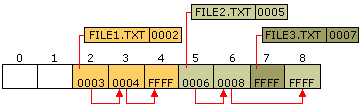
\includegraphics[width=0.5\linewidth, center]{pics/31fat.png}
	    \begin{itemize}
           \pause\item Файл состоит из цепочки блоков
           \pause\item Последовательная цепочка блоков файла - фрагмент
           \pause\item В идеале - 1 фрагмент, но их может быть много (тема отдельной презентации)
        \end{itemize}
}

\frame {
	    \frametitle{Эксперимент}
	    \framesubtitle{Постановка вопроса}
	\pause Как понять, что мы...
	\begin{itemize}
    \pause\item \sout{в матрице?}
    \pause\item \sout{в квантовом мире?}
    \pause\item файл на самом деле имеет блочную структуру?
    \end{itemize}
    \vspace{0.5cm}
    \pause А вот как! Будем читать два байта! Причём два раза:
    \begin{itemize}
    \pause\item Внутри блока - как baseline
    \pause\item На границе двух блоков - должно быть медленнее
    \end{itemize}
    \vspace{0.5cm}
    \pause Назовём этот эксперимент "Как два байта почитать".
}
\frame {
	    \frametitle{Эксперимент: Как два байта почитать}
	    \framesubtitle{Уточнения}
    \pause Остаётся вопрос. А какой реальный размер блока?\\
    \begin{itemize}
    \pause\item Когда как... Обычно всё пляшет вокруг 4096 байт. Но это не точно. Будем перебирать несколько вариантов: 128, 256, ..., 524288.
    \end{itemize}
    \vspace{0.5cm}
    \pause А также второй вопрос. А размер блока чего? Устройства хранения? Файловой системы? Страницы памяти?
    \begin{itemize}
    \pause\item Не важно. Все они пляшут вокруг 4096. Если отличаются, то сможем напороться сразу на несколько аномалий.
    \end{itemize}
}

\frame {
	    \frametitle{Эксперимент: Как два байта почитать}
	    \framesubtitle{Спецификации стенда и эксперимента}
    \pause Hardware
    \begin{itemize}
     \item {\bf HDD/SATA}: 500GB Hitachi, 8MB, 5400RPM, 10ms/300IOps {\scriptsize (HTS545050B9A300)}
     \item {\bf SSD/SATA}: 500GB Samsung 850 EVO, 512MB, 90{\bf K}IOps {\scriptsize(MZ-75E500BW)}
     \item {\bf SSD/NVMe}: 512GB Samsung 960 PRO, 512MB, 500{\bf K}IOps {\scriptsize(MZ-V7P512BW)}
    \end{itemize}
    \pause Software
    \begin{itemize}
     \item {\bf OS}: GNU/Linux (Gentoo)
     \item {\bf FS}: BTRFS
     \item {\bf Runtime}: .Net Core v3.1 + FileStream.Read
    \end{itemize}
    \pause Calculus
    \begin{itemize}
     \item Все чтения с устройств были случайными, за время итерации каждый блок читался не более одного раза
     \item Для SSD делалось 1000, для HDD - 40 измерений на точку
     \item 5\% выбросов в обе стороны отбрасывалось, результат усреднялся
    \end{itemize}
}

\frame {
\frametitle{Эксперимент: Как два байта почитать}
\framesubtitle{Отсутствие результата - тоже результат}
\begin{columns}
 \begin{column}[c]{0.50\paperwidth}
  \begin{minipage}[c]{1\textwidth}
   \colorbox{white}{\includegraphics[width=\textwidth]{../data/hdd-file-single.pdf}}
  \end{minipage}
  \end{column}
 \begin{column}[c]{0.40\paperwidth}
 Здесь и далее на графиках: Время чтения 2 байт (в мс) на гипотетической границе двух блоков от размера блока (в байтах).\\
\vspace{1cm}
\pause
HDD: Ничего интересного не видно. Муть какая-то...
 \end{column}
\end{columns}
}
\frame {
\frametitle{Эксперимент: Как два байта почитать}
\framesubtitle{Есть рывок!}
\begin{columns}
 \begin{column}[c]{0.50\paperwidth}
  \begin{minipage}[c]{1\textwidth}
   \colorbox{white}{\includegraphics[width=\textwidth]{../data/ssd-file-single.pdf}}
  \end{minipage}
  \end{column}
 \begin{column}[c]{0.40\paperwidth}
SSD/SATA: Есть рывок на 4096 КБ!
 \end{column}
\end{columns}
}
\frame {
\frametitle{Эксперимент: Как два байта почитать}
\framesubtitle{Ещё рывок!}
\begin{columns}
 \begin{column}[c]{0.50\paperwidth}
  \begin{minipage}[c]{1\textwidth}
   \colorbox{white}{\includegraphics[width=\textwidth]{../data/nvm-file-single.pdf}}
  \end{minipage}
  \end{column}
 \begin{column}[c]{0.40\paperwidth}
SSD/SATA: Есть рывок на 4096 КБ!
 \end{column}
\end{columns}
}

\frame {
\frametitle{Эксперимент: Как два байта почитать}
\framesubtitle{Сводная табличка}
\begin{columns}
 \begin{column}[c]{0.50\paperwidth}
  \begin{minipage}[c]{1\textwidth}
   \colorbox{white}{\includegraphics[width=\textwidth]{../data/file-compose.pdf}}
  \end{minipage}
  \end{column}
 \begin{column}[c]{0.40\paperwidth}
 \begin{itemize}
    \item 20мс - время чтения хуже в два раза спецификации нашего HDD
    \item SSD круче HDD на два порядка
    \item NVMe быстрее SATA в 2 раза
 \end{itemize}
 \end{column}
\end{columns}
}

\frame {
\frametitle{Эксперимент: Как два байта почитать}
\framesubtitle{Всем спасибо}
\begin{center}
Всё, расходимся.
\end{center}
}

\frame {
\frametitle{Эксперимент: Как два байта почитать}
\framesubtitle{Всем спасибо}
\begin{center}
Нет, постойте!
\end{center}
}

\frame {
\frametitle{Эксперимент: Как два байта почитать}
\framesubtitle{Но это ещё не всё!}
\begin{columns}
 \begin{column}[c]{0.50\paperwidth}
  \begin{minipage}[c]{1\textwidth}
   \colorbox{white}{\includegraphics[width=\textwidth]{../data/hdd-file-single.pdf}}
  \end{minipage}
  \end{column}
 \begin{column}[c]{0.40\paperwidth}
 Эту картинку вы уже видели
 \end{column}
\end{columns}
}

\frame {
\frametitle{Эксперимент: Как два байта почитать}
\framesubtitle{Но это ещё не всё!}
\begin{columns}
 \begin{column}[c]{0.50\paperwidth}
  \begin{minipage}[c]{1\textwidth}
   \colorbox{white}{\includegraphics[width=\textwidth]{../data/hdd-file-caching-2.pdf}}
  \end{minipage}
  \end{column}
 \begin{column}[c]{0.40\paperwidth}
 У нас нет воспроизводимого результата!
 \end{column}
\end{columns}
}

\frame {
\frametitle{Эксперимент: Как два байта почитать}
\framesubtitle{Но это ещё не всё!}
\begin{columns}
 \begin{column}[c]{0.50\paperwidth}
  \begin{minipage}[c]{1\textwidth}
   \colorbox{white}{\includegraphics[width=\textwidth]{../data/hdd-file-caching-3.pdf}}
  \end{minipage}
  \end{column}
 \begin{column}[c]{0.40\paperwidth}
 У нас нет воспроизводимого результата!\\
\vspace{1cm} 
 Это не эксперимент. Это - ерунда какая-то.
 \end{column}
\end{columns}
}

\frame {
\frametitle{Эксперимент: Как два байта почитать}
\framesubtitle{Но это ещё не всё!}
\begin{columns}
 \begin{column}[c]{0.50\paperwidth}
  \begin{minipage}[c]{1\textwidth}
   \colorbox{white}{\includegraphics[width=\textwidth]{../data/hdd-file-caching.pdf}}
  \end{minipage}
  \end{column}
 \begin{column}[c]{0.40\paperwidth}
   
\includegraphics[width=\textwidth]{pics/fine2.jpg}
 \end{column}
\end{columns}
}

\frame {
\frametitle{Эксперимент: Как два байта почитать}
\framesubtitle{Но это ещё не всё!}
\begin{columns}
 \begin{column}[c]{0.50\paperwidth}
  \begin{minipage}[c]{1\textwidth}
   \colorbox{white}{\includegraphics[width=\textwidth]{../data/ssd-file-caching.pdf}}
  \end{minipage}
  \end{column}
 \begin{column}[c]{0.40\paperwidth}
   
\includegraphics[width=\textwidth]{pics/fine2.jpg}
 \end{column}
\end{columns}
}

\frame {
\frametitle{Эксперимент: Как два байта почитать}
\framesubtitle{Но это ещё не всё!}
\begin{columns}
 \begin{column}[c]{0.50\paperwidth}
  \begin{minipage}[c]{1\textwidth}
   \colorbox{white}{\includegraphics[width=\textwidth]{../data/nvm-file-caching.pdf}}
  \end{minipage}
  \end{column}
 \begin{column}[c]{0.40\paperwidth}
   
\includegraphics[width=\textwidth]{pics/fine2.jpg}
 \end{column}
\end{columns}
}

\frame {
\frametitle{Эксперимент: Как два байта почитать}
\framesubtitle{Разгадка загадки}
\begin{columns}
 \begin{column}[c]{0.50\paperwidth}
  \begin{minipage}[c]{1\textwidth}
   \colorbox{white}{\includegraphics[width=\textwidth]{../data/nvm-file-caching.pdf}}
  \end{minipage}
  \end{column}
 \begin{column}[c]{0.40\paperwidth}
   Кэширование файла операционной системой!!!\\
   \vspace{1cm}
   \pause ... или файловой системой?\\
   \vspace{1cm}
   \pause ... или кэш устройства?\\
   \vspace{1cm}
   \pause ... \sout{ну или кэш браузера!?}\\
 \end{column}
\end{columns}
}

\frame {
\frametitle{Эксперимент: Как два байта почитать}
\framesubtitle{Разгадка загадки}
    \begin{itemize}
     \pause\item {\normalsize Почему загиб при больших размерах блока?\\\pause \hspace{0.8cm} - объяснимо. Действительно, где-то кэш. Число больших блоков маленькое, чаще читается, больше вероятности попасть в кэш}
     \vspace{0.5cm}
     \pause\item {\normalsize Почему для HDD нет загиба?\\\pause \hspace{0.8cm} - объяснимо. Для HDD делалось всего 40 замеров на точку, для SSD - 1000. Просто успевало прокэшироваться. Действительно, если делать больше замеров, то загиб у HDD также появляется}
     \vspace{0.5cm}\pause\item {\normalsize Чей кэш? \pause - \alert{с этим сложно...}}
    \end{itemize}
}

\frame {
\frametitle{Эксперимент: Как два байта почитать}
\framesubtitle{Так чей кэш?}
Мы в линкусе!\\
\vspace{0.1cm}
\pause\hspace{0.2\textwidth}\tt{\bf umount/mount}\\
\pause\vspace{0.2cm} \hfill - Кэш сбрасывается! Значит он был в файловой системе. Или в OS. Не суть.
}

\frame {
\frametitle{Эксперимент: Как два байта почитать}
\framesubtitle{Deeper... deeper!!!}
Копнём глубже. \pause Мы в линкусе! \pause \tt{new FileStream("{\bf /dev/sdc}")} !!!
}

\frame {
\frametitle{Эксперимент: Как два байта почитать}
\framesubtitle{Deeper... deeper!!!}
\begin{columns}
 \begin{column}[c]{0.50\paperwidth}
  \begin{minipage}[c]{1\textwidth}
   \colorbox{white}{\includegraphics[width=\textwidth]{../data/hdd-raw-single.pdf}}
  \end{minipage}
  \end{column}
 \begin{column}[c]{0.40\paperwidth}
    \begin{itemize}
     \item Быстрее в 2 раза!
     \item Но граница блока не прощупывается
    \end{itemize}
 \end{column}
\end{columns}
}

\frame {
\frametitle{Эксперимент: Как два байта почитать}
\framesubtitle{Deeper... deeper!!!}
\begin{columns}
 \begin{column}[c]{0.50\paperwidth}
  \begin{minipage}[c]{1\textwidth}
   \colorbox{white}{\includegraphics[width=\textwidth]{../data/ssd-raw-single.pdf}}
  \end{minipage}
  \end{column}
 \begin{column}[c]{0.40\paperwidth}
    \begin{itemize}
     \item Быстрее в 2 раза
     \item Граница блока прощупывается на 4096
    \end{itemize}
 \end{column}
\end{columns}
}

\frame {
\frametitle{Эксперимент: Как два байта почитать}
\framesubtitle{Deeper... deeper!!!}
\begin{columns}
 \begin{column}[c]{0.50\paperwidth}
  \begin{minipage}[c]{1\textwidth}
   \colorbox{white}{\includegraphics[width=\textwidth]{../data/nvm-raw-single.pdf}}
  \end{minipage}
  \end{column}
 \begin{column}[c]{0.40\paperwidth}
    \begin{itemize}
     \item Быстрее в 2 раза
     \item Граница блока прощупывается на 4096
    \end{itemize}
 \end{column}
\end{columns}
}

\frame {
\frametitle{Эксперимент: Как два байта почитать}
\framesubtitle{Deeper... deeper!!!}
\begin{columns}
 \begin{column}[c]{0.50\paperwidth}
  \begin{minipage}[c]{1\textwidth}
   \colorbox{white}{\includegraphics[width=\textwidth]{../data/raw-compose.pdf}}
  \end{minipage}
  \end{column}
 \begin{column}[c]{0.40\paperwidth}
    \begin{itemize}
     \item Расклад не изменился, все просто стали в 2 раза быстрее
     \item HDD даёт 10мс на чтение, что гарантировано спецификацией
    \end{itemize}
 \end{column}
\end{columns}
}

\frame {
\frametitle{Эксперимент: Как два байта почитать}
\framesubtitle{Deeper... deeper!!! Caching!!!!!}
\begin{columns}
 \begin{column}[c]{0.60\paperwidth}
 \hfill \huge Мы победили кэширование!
   \end{column}
 \begin{column}[c]{0.40\paperwidth}
 \hspace{1cm} \Huge \color{gray2} ДА!!! :)
  \end{column}
\end{columns}
}

\frame {
\frametitle{Эксперимент: Как два байта почитать}
\framesubtitle{Deeper... deeper!!! Caching!!!!!}
\begin{columns}
 \begin{column}[c]{0.60\paperwidth}
 \hfill \huge Мы победили кэширование!?
   \end{column}
 \begin{column}[c]{0.40\paperwidth}
 \hspace{1cm} \Huge \bf Нет :(
  \end{column}
\end{columns}
}

\frame {
\frametitle{Эксперимент: Как два байта почитать}
\framesubtitle{Deeper... deeper!!!}
\begin{columns}
 \begin{column}[c]{0.50\paperwidth}
  \begin{minipage}[c]{1\textwidth}
   \colorbox{white}{\includegraphics[width=\textwidth]{../data/ssd-raw-caching.pdf}}
  \end{minipage}
  \end{column}
 \begin{column}[c]{0.50\paperwidth}
  \begin{minipage}[c]{1\textwidth}
   \colorbox{white}{\includegraphics[width=\textwidth]{../data/nvm-raw-caching.pdf}}
  \end{minipage}
 \end{column}
\end{columns}
}

\frame {
\frametitle{Выводы}
\framesubtitle{Всё сложно}
\begin{itemize}
\pause\item Да, в рамках блока в 4096 байт данные читаются быстрее (для SSD)
\pause\item Нет, затачиваться на границу в 4096 смысла особого нет, т.к. разница в скорости всего 10\%, а не в два раза
\pause\item В HDD разница не обнаржена. Видимо из-за того, что была низкая фрагментация файла
\pause\item При бенчмарках на файлах очень не просто добиться воспроизводимого результата. Кэшируется всё подряд
\pause\item Планировалось два эксперимента, а получилось как всегда - один. И тот ни о чём
\pause\item Делать презентации в \LaTeX  - это практично, молодёжно. Здоровья вам!
\end{itemize}
}


\end{document}
